\documentclass[english,twoside]{article}

\input{../../131/StudentGuideModule1/labmanual_formatting_commands} %all general latex packages, commands, and definitions now here.
\newcommand{\coursefolder}{Relativity~FYS} %This defines the place students will look for various files
\ForceSectionOddPage %This option makes each lab start on odd numbered page (right hand side).

%The \includeonly line below is a great way to save time so you don't always have to compile the WHOLE latex document, if for instance you've only made changes to a single lab.  If you want to compile more than two labs, the syntax is \includeonly{lab1,lab2,lab3} with no spaces after the commas.
%The master.pdf produced will have only the title page, TOC, and that single lab, though the other lab names will appear in the TOC.
%\includeonly{binomial_expansion/binomial_expansion}

%Use the following line to override all of the 1's and 0's in the \includelab statements below
%\includealllabstrue

%Use the line below to disable hyperlinks, to make sure no markups are visible around references when printing.
\hypersetup{draft}

\usepackage{isotope}
\usepackage{eso-pic}
\usepackage{atbegshi}
\usepackage{pdflscape}
\usepackage{pdfpages}
\usepackage[lastexercise,answerdelayed]{exercise}
\usepackage{chngcntr}
\usepackage{upgreek}
\renewcommand{\gamma}{\upgamma}
%\renewcommand{\numberline}[1]{#1~}

\makeatletter
\newcommand{\cftlotnumberline}[1]{\@cftbsnum #1\@cftasnum\@cftasnumb}
\makeatother



\makeindex
\begin{document}


\index{color page}

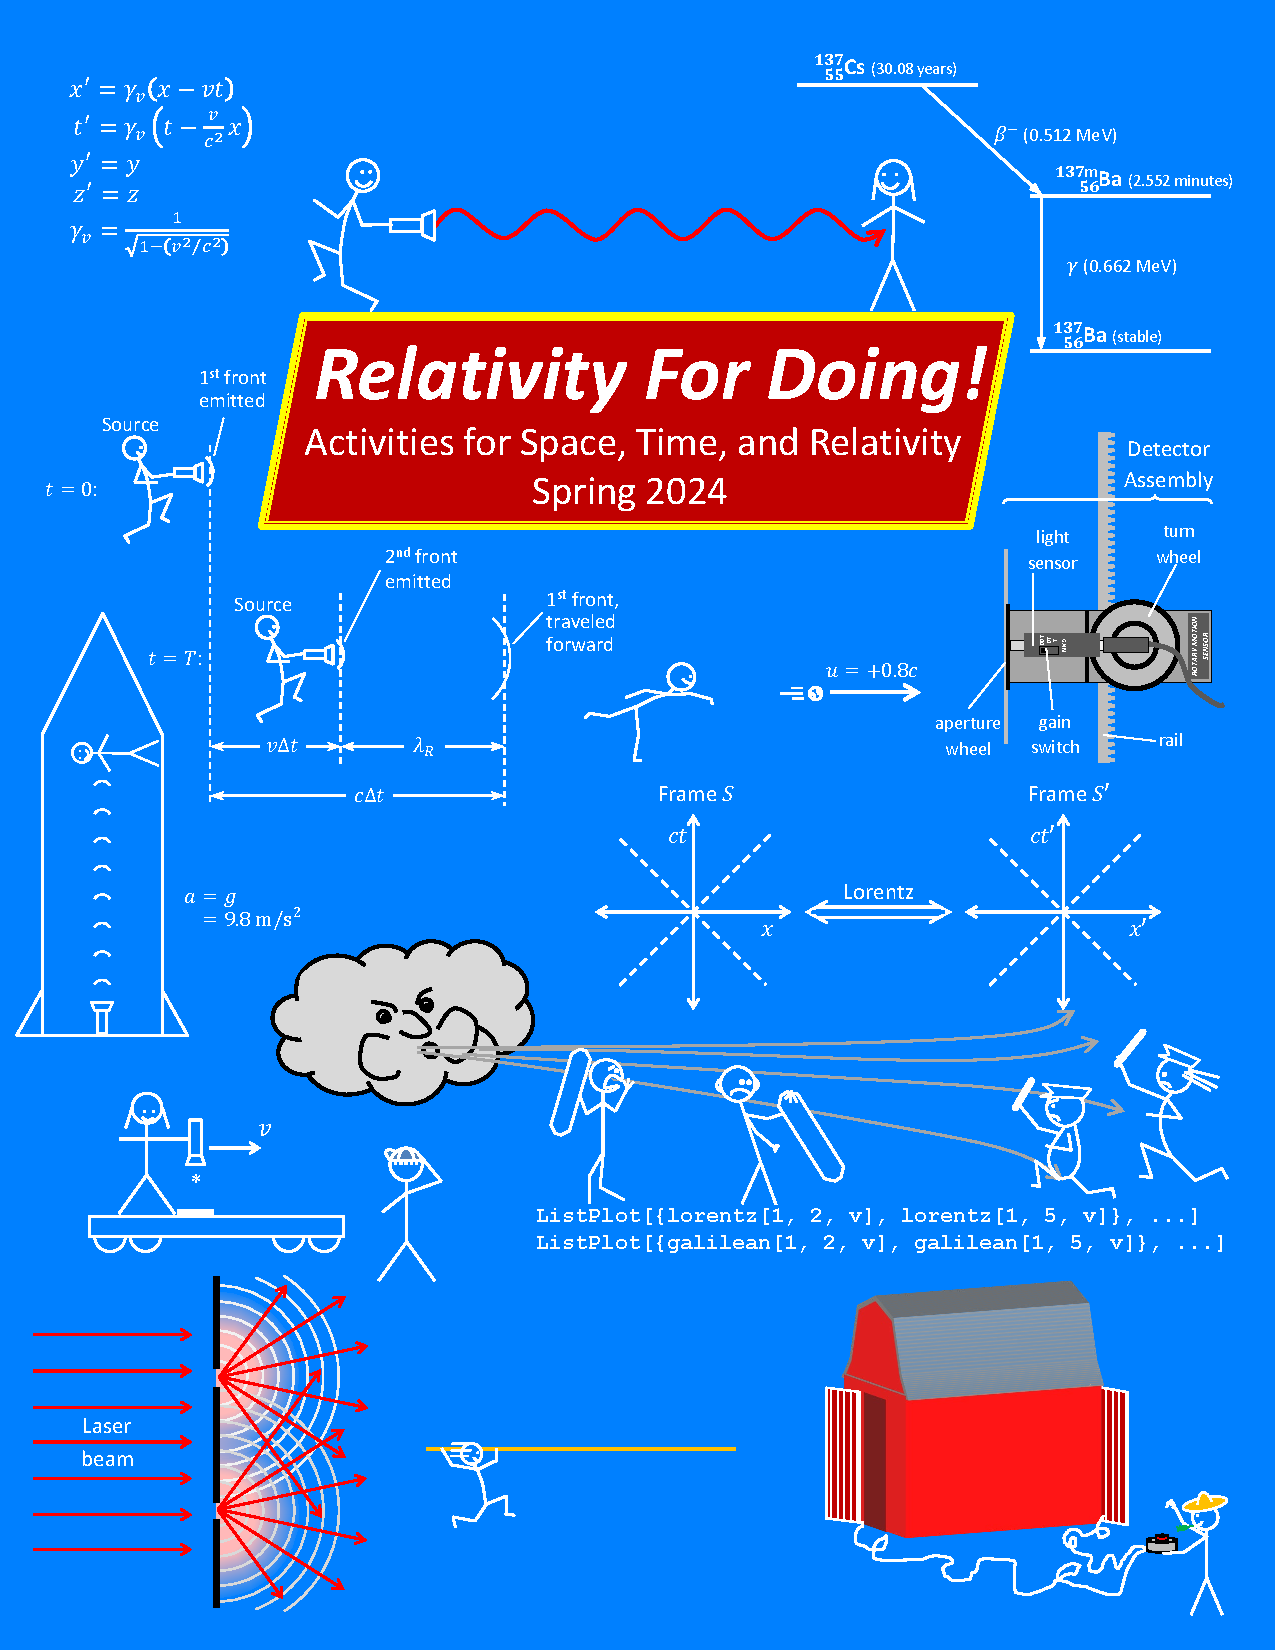
\includepdf[pages=1]{FYS_front_pages/FYS_front_cover.pdf}

\thispagestyle{empty}

\

\vfill
\textit{Cover art: Various graphics and diagrams from the activities in this manual.  You'll be doing lots of stuff.}
\pagebreak



\title{Relativity For Doing!\\
Activities for First-Year Seminar: Space, Time, and Relativity}

%\author{Gerard P. Gilfoyle}
%\author{Jack Singal}
% MT sez: I think I wrote all of the relativity labs that we're going to do here... 
% Jerry wrote the original Nuclear Physics lab.
% From the other lab manuals, I think I'll only use the Doppler effect lab and the two-slit interference lab,
% which I also wrote the current version of.  Happy to add another author if I'm missing anything...
\author{Matthew L. Trawick}
\affil{Department of Physics, University of Richmond, VA}

\maketitle

\vspace{0.8 in}

%\begin{abstract}

\begin{center}
\large{\textbf{Welcome to Space, Time, and Relativity!}}
\end{center}


This manual is a set of exercises for use in the First-Year Seminar section ``Space, Time, and Relativity'' at the University of Richmond, covering various topics in special and general relativity.  These exercises are primarily intended as in-class activities, or ``labs,'' though most of them are kind of fake labs in that they don't use any physical equipment beyond a computer and some software, at most.

MT gratefully acknowledges the advice and assistance of Ted Bunn, both for fielding specific Mathematica questions and for many helpful discussions about teaching this course.

%\end{abstract}


\newpage
\
\thispagestyle{plain}

\newpage
\

%\renewcommand{\sectionmark}[1]{\markboth{\MakeUppercase{\chaptername\ WOO \thechapter.\ #1}}{}}
\renewcommand{\sectionmark}[1]{\markboth{\MakeUppercase{\thesection:\ #1}}{}}

\fancyhead[LE,RO]{\slshape \MakeUppercase{CONTENTS}\leftmark}
\renewcommand{\part}[1]{
	\stepcounter{tocpartnum}
	\phantomsection %This line fixes a problem in compiling the "bookmarks" (the outline) in hyperref under pdflatex.
	\immediateaddcontentsline{toc}{part}{Part \Alph{tocpartnum}:\hspace{1ex}#1}{}}
\setlength{\cftsubsecnumwidth}{1.6em}
\setlength{\cftsecnumwidth}{1.0em}
\renewcommand{\cftmarktoc}{}
\renewcommand{\cftsubsecaftersnumb}{~Problems:~}
\renewcommand{\cftsecpresnum}{\headersupplementmark}
\renewcommand{\cftsecpresnum}{Appendix~}
\renewcommand{\cftsecaftersnumb}{:~}
\setcounter{tocdepth}{2}
\let\numberline\cftlotnumberline
\tableofcontents{}
\cleardoublepage
\pagestyle{labfancy}

%Use \includelab{1} to include, or \includelab{0} to exclude.  Overridden with \includealllabstrue or \includeonly
%--------------------------------------------
\part{Physics Before Einstein 1: Waves and Velocity}

\includelab{1}[../../132/StudentGuideModule2/]{interference_of_light/interference} %Matt's Version
\includelab{1}[../../131/StudentGuideModule1/]{position/position}

\part{Physics Before Einstein 2: Galilean Relativity}

\includelab{1}[../../131/StudentGuideModule1/]{galilean_exercises/galilean_exercises}
\includelab{1}{swimming_race/swimming_race}
\includelab{1}{sound_vs_baseballs/sound_vs_baseballs}

%--------------------------------------------
\part{Time, Length, and Lorentz Transformations}

\includelab{1}[../../131/StudentGuideModule1/]{time_dilation_length_contraction/time_dilation_length_contraction} 
\includelab{1}{binomial_expansion/binomial_expansion}
\includelab{1}[../../131/StudentGuideModule1/]{lorentz_transformations/lorentz_transformations}
\includelab{1}{messing_with_lorentz/messing_with_lorentz} 


%--------------------------------------------
\part{Gravitation and General Relativity}

\includelab{1}[../../131/StudentGuideModule1/]{gravity_normal_elevators/gravity_normal_elevators}
\includelab{1}{gravity_time/gravity_time}

%--------------------------------------------
\part{Velocity, Speed of Light, and Causality}

\includelab{1}{velocity_transformations/velocity_transformations} 
\includelab{1}{faster_than_light/faster_than_light} 
\includelab{0}{proper_length_distance/proper_length_distance}

%--------------------------------------------
\part{Energy and Mass}

\includelab{1}{energy_mass/energy_mass_warmups}
\includelab{1}{energy_mass/relativistic_energy_mass}

%--------------------------------------------
\part{More Examples}

\includelab{1}[../../132/StudentGuideModule2/]{radiocarbon_dating/radiocarbon_dating_simplified}
\includelab{1}[../../131/StudentGuideModule1/]{time_dilation_length_contraction/muon_lifetimes}
\includelab{1}[../../131/StudentGuideModule1/]{pole_and_barn/pole_and_barn} 
\includelab{1}{twin_paradox/twin_paradox}
\includelab{0}[../../132/StudentGuideModule2/]{doppler_shift/doppler_shift}
\includelab{0}{relativistic_doppler/relativistic_doppler}

\includelab{0}{relativistic_example/relativistic_example}

%--------------------------------------------
\startappendix
\renewcommand{\cftsecpresnum}{Appendix:~}


\includelab{1}{appendices/units_and_prefixes}
\includelab{1}{appendices/greek_letters}
\includelab{1}{appendices/nuclear_primer}
\includelab{1}[../../131/StudentGuideModule1/]{appendices/capstone/capstone}
\includelab{1}{relativistic_boot_camp/relativistic_boot_camp}

\includelab{0}[../../132/StudentGuideModule2/]{appendices/nuke_safety/nuke_safety}
\setcounter{section}{12}
\renewcommand{\thesubsection}{\thesection\Alph{subsection}}
\includelab{0}{M_problems/M_problems}
\includelab{1}{M_problems/M_problems_latex}

% The following command prints the "Instructor Notes" section at the end of the manual.
% Comment it out for the regular student edition.
%\startinstructornotes
\end{document}
